\documentclass[12pt]{article}
\usepackage{graphicx}
\usepackage[margin=2cm]{geometry}
\usepackage[utf8]{inputenc}
\usepackage{tikz}
\usepackage[export]{adjustbox}
\usepackage{indentfirst}
\usepackage{wrapfig}
\usepackage{listings}
\usepackage{color}
\usepackage{enumerate}
\usepackage{amssymb, bm}
\usepackage{amsmath}
\usepackage{csvsimple}
\usepackage{tikz}
\usetikzlibrary{positioning}
\usepackage{lscape}
\newcommand\tab[1][1cm]{\hspace*{#1}}
\definecolor{mygreen}{rgb}{0,0.6,0}
\definecolor{mygray}{rgb}{0.5,0.5,0.5}
\definecolor{mymauve}{rgb}{0.58,0,0.82}
\lstset{ %
    backgroundcolor=\color{gray!10!white},
  basicstyle=\tiny, %footnotesize,        % the size of the fonts that are used for the code
  breakatwhitespace=false,         % sets if automatic breaks should only happen at whitespace
  breaklines=true,                 % sets automatic line breaking
  captionpos=b,                    % sets the caption-position to bottom
  commentstyle=\color{mygreen},    % comment style
  deletekeywords={...},            % if you want to delete keywords from the given language
  escapeinside={\%*}{*)},          % if you want to add LaTeX within your code
  extendedchars=true,              % lets you use non-ASCII characters; for 8-bits encodings only, does not work with UTF-8
  frame=single,	                   % adds a frame around the code
  keepspaces=true,                 % keeps spaces in text, useful for keeping indentation of code (possibly needs columns=flexible)
  keywordstyle=\color{blue},       % keyword style
  language=Python,                 % the language of the code
  morekeywords={*,...},           % if you want to add more keywords to the set
  numbers=left,                    % where to put the line-numbers; possible values are (none, left, right)
  numbersep=10pt,                   % how far the line-numbers are from the code
  numberstyle=\tiny\color{mygray}, % the style that is used for the line-numbers
  rulecolor=\color{black},         % if not set, the frame-color may be changed on line-breaks within not-black text (e.g. comments (green here))
  showspaces=false,                % show spaces everywhere adding particular underscores; it overrides 'showstringspaces'
  showstringspaces=false,          % underline spaces within strings only
  showtabs=false,                  % show tabs within strings adding particular underscores
  stepnumber=1,                    % the step between two line-numbers. If it's 1, each line will be numbered
  stringstyle=\color{mymauve},     % string literal style
  tabsize=1,	                   % sets default tabsize to 2 spaces
  title=\lstname                   % show the filename of files included with \lstinputlisting; also try caption instead of title
}
\graphicspath{ }
\usetikzlibrary{arrows}

\title{\textbf{COMP0085 Summative Assignment}}
%\author{Jian Shu (James) Wu \\ }
\date{Jan 4, 2023}

\begin{document}
\maketitle
\section*{Question 1}

\subsection*{(a)} The directed acyclic graph:

\begin{center}
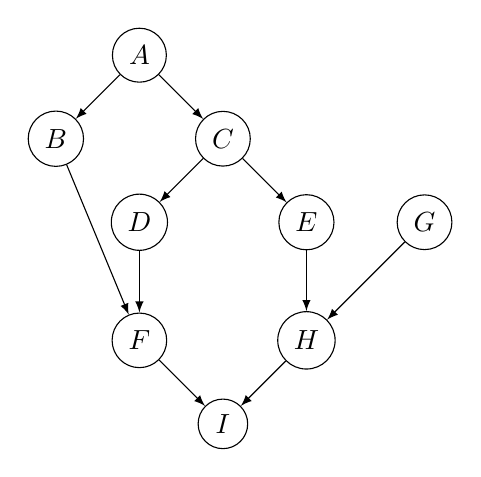
\begin{tikzpicture}[node distance={15mm}, main/.style = {draw, circle}]
    \node[main] (A) {$A$};
    \node[main] (B) [below left of=A] {$B$};
    \node[main] (C) [below right of=A] {$C$};
    \node[main] (E) [below right of=C] {$E$};
    \node[main] (D) [below left of=C] {$D$};
    \node[main] (H) [below of=E] {$H$};
    \node[main] (G) [right of=E] {$G$};
    \node[main] (I) [below left of=H] {$I$};
    \node[main] (F) [above left of=I] {$F$};

    \draw[-latex] (A) -- (B);
    \draw[-latex] (A) -- (C);
    \draw[-latex] (B) -- (F);
    \draw[-latex] (C) -- (D);
    \draw[-latex] (C) -- (E);
    \draw[-latex] (G) -- (H);
    \draw[-latex] (D) -- (F);
    \draw[-latex] (E) -- (H);
    \draw[-latex] (F) -- (I);
    \draw[-latex] (H) -- (I);
\end{tikzpicture}
\end{center}

\newpage


\subsection*{(b)} The moralised graph:

\begin{center}
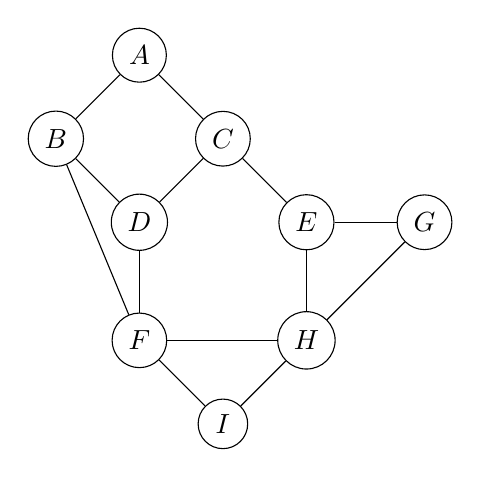
\begin{tikzpicture}[node distance={15mm}, main/.style = {draw, circle}]
    \node[main] (A) {$A$};
    \node[main] (B) [below left of=A] {$B$};
    \node[main] (C) [below right of=A] {$C$};
    \node[main] (E) [below right of=C] {$E$};
    \node[main] (D) [below left of=C] {$D$};
    \node[main] (H) [below of=E] {$H$};
    \node[main] (G) [right of=E] {$G$};
    \node[main] (I) [below left of=H] {$I$};
    \node[main] (F) [above left of=I] {$F$};

    \draw (A) -- (B);
    \draw (A) -- (C);
    \draw (B) -- (F);
    \draw (B) -- (D);
    \draw (C) -- (D);
    \draw (C) -- (E);
    \draw (E) -- (G);
    \draw (G) -- (H);
    \draw (D) -- (F);
    \draw (E) -- (H);
    \draw (F) -- (H);
    \draw (F) -- (I);
    \draw (H) -- (I);
\end{tikzpicture}
\end{center}


An effective triangulation:


\begin{center}
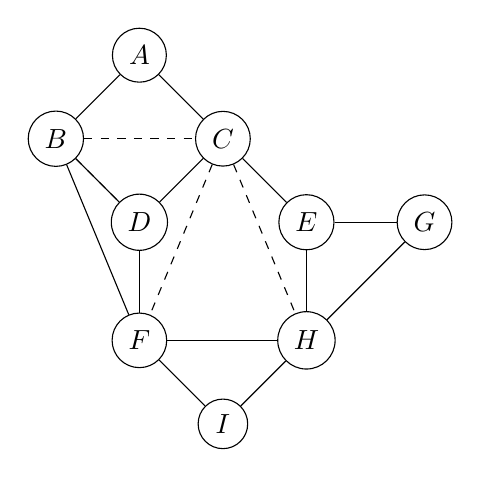
\begin{tikzpicture}[node distance={15mm}, main/.style = {draw, circle}]
    \node[main] (A) {$A$};
    \node[main] (B) [below left of=A] {$B$};
    \node[main] (C) [below right of=A] {$C$};
    \node[main] (E) [below right of=C] {$E$};
    \node[main] (D) [below left of=C] {$D$};
    \node[main] (H) [below of=E] {$H$};
    \node[main] (G) [right of=E] {$G$};
    \node[main] (I) [below left of=H] {$I$};
    \node[main] (F) [above left of=I] {$F$};

    \draw (A) -- (B);
    \draw (A) -- (C);
    \draw (B) -- (F);
    \draw (B) -- (D);
    \draw (C) -- (D);
    \draw (C) -- (E);
    \draw (E) -- (G);
    \draw (G) -- (H);
    \draw (D) -- (F);
    \draw (E) -- (H);
    \draw (F) -- (H);
    \draw (F) -- (I);
    \draw (H) -- (I);

    \draw[dashed] (C) -- (H);
    \draw[dashed] (C) -- (F);
    \draw[dashed] (B) -- (D);
    \draw[dashed] (B) -- (C);

\end{tikzpicture}
\end{center}

where the dashed lines are edges added to triangulate the moralised graph.
\newpage


The resulting junction tree:



%\begin{center}
%\begin{tikzpicture}[node distance={25mm}, main/.style = {draw, circle}, square/.style={regular polygon,regular polygon sides=4}]
%    \node[main] (ABC) {$ABC$};
%    \node[main] (BCDF) [below of=ABC] {$BCDF$};
%    \node[main] (CFH) [below of=BCDF] {$CFH$};
%    \node[main] (FHI) [below left of=CFH] {$FHI$};
%    \node[main] (CEH) [below right of=CFH] {$CEH$};
%    \node[main] (EGH) [below of=CEH] {$EGH$};
%    \draw (ABC) -- (BCDF);
%    \draw (BCDF) -- (CFH);
%    \draw (CFH) -- (FHI);
%    \draw (CFH)  -- (CEH);
%    \draw (EGH)  -- (CEH);
%\end{tikzpicture}
%\end{center}

\begin{center}
\begin{tikzpicture}[node distance={15mm}, main/.style = {draw, circle}, square/.style={regular polygon,regular polygon sides=4}]
    \node[main] (ABC) {$ABC$};
    \node[square] (BC) [square,draw] [below of=ABC] {$BC$};
    \node[main] (BCDF) [below of=BC] {$BCDF$};
    \node[square] (CF) [square,draw] [below of=BCDF] {$CF$};
    \node[main] (CFH) [below of=CF] {$CFH$};
    \node[square] (FH) [square,draw] [below left of=CFH] {$FH$};
    \node[main] (FHI) [below left of=FH] {$FHI$};
    \node[square] (CH) [square,draw] [below right of=CFH] {$CH$};
    \node[main] (CEH) [below right of=CH] {$CEH$};
    \node[square] (EH) [square,draw] [below of=CEH] {$EH$};
    \node[main] (EGH) [below of=EH] {$EGH$};
    \draw (ABC) -- (BC);
    \draw (BC) -- (BCDF);
    \draw (BCDF) -- (CF);
    \draw (CF) -- (CFH);
    \draw (CFH) -- (FH);
    \draw (FH) -- (FHI);
    \draw (CFH) -- (CH);
    \draw (CH) -- (CEH);
    \draw (CEH) -- (EH);
    \draw (EGH) -- (EH);
\end{tikzpicture}
\end{center}

where the circular nodes are cliques and the square nodes are separators/factors.


The junction tree redrawn as a factor graph:

\begin{center}
\begin{tikzpicture}[node distance={10mm}, main/.style = {draw, circle}, square/.style={fill=black, regular polygon,regular polygon sides=4}]
    \node[main] (A) {$A$};
    \node[square] (ABC) [square,draw] [below of=A];
    \node[main] (B) [below left of=ABC] {$B$};
    \node[main] (C) [below right of=ABC] {$C$};
    \node[square] (BCDF) [square,draw] [below left of=C];
    \node[square] (CEH) [right of=C];
    \node[main] (E) [above right of=CEH] {$E$};
    \node[square] (GEH) [below right of=E];
    \node[main] (G) [right of=GEH] {$G$};
    \node[main] (D) [below left of=BCDF] {$D$};
    \node[square] (CFH) [below right of=C];
    \node[main] (H) [right of=CFH] {$H$};
    \node[square] (FHI) [below left of = H];
    \node[main] (I) [below right of=FHI] {$I$};
    \node[main] (F) [below right of=BCDF] {$F$};

    \draw (ABC) -- (A);
    \draw (ABC) -- (C);
    \draw (ABC) -- (B);
    \draw (BCDF) -- (B);
    \draw (BCDF) -- (C);
    \draw (BCDF) -- (D);
    \draw (BCDF) -- (F);
    \draw (CEH) -- (C);
    \draw (CEH) -- (E);
    \draw (CEH) -- (H);
    \draw (GEH) -- (G);
    \draw (GEH) -- (E);
    \draw (GEH) -- (H);
    \draw (CFH) -- (C);
    \draw (CFH) -- (F);
    \draw (CFH) -- (H);
    \draw (FHI) -- (F);
    \draw (FHI) -- (H);
    \draw (FHI) -- (I);
\end{tikzpicture}
\end{center}
\newpage


\subsection*{(c)}

\begin{center}
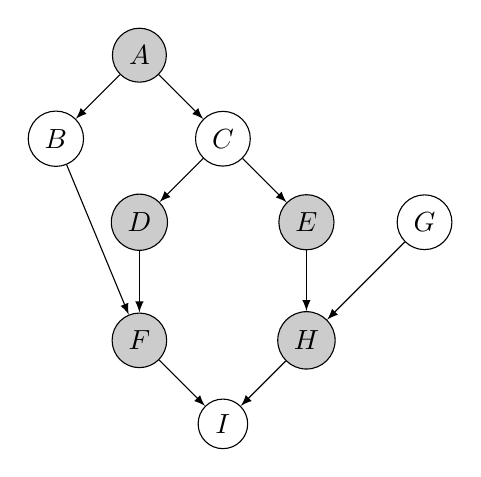
\begin{tikzpicture}[node distance={15mm}, main/.style = {draw, circle}]
    \node[main] (A) [fill=black!20] {$A$};
    \node[main] (B) [below left of=A] {$B$};
    \node[main] (C) [below right of=A] {$C$};
    \node[main] (E) [below right of=C, fill=black!20] {$E$};
    \node[main] (D) [below left of=C, fill=black!20] {$D$};
    \node[main] (H) [below of=E, fill=black!20] {$H$};
    \node[main] (G) [right of=E] {$G$};
    \node[main] (I) [below left of=H] {$I$};
    \node[main] (F) [above left of=I, fill=black!20] {$F$};

    \draw[-latex] (A) -- (B);
    \draw[-latex] (A) -- (C);
    \draw[-latex] (B) -- (F);
    \draw[-latex] (C) -- (D);
    \draw[-latex] (C) -- (E);
    \draw[-latex] (G) -- (H);
    \draw[-latex] (D) -- (F);
    \draw[-latex] (E) -- (H);
    \draw[-latex] (F) -- (I);
    \draw[-latex] (H) -- (I);
\end{tikzpicture}
\end{center}


The set $\{A, D, E, F, H\}$ is a non-unique smallest set of molecules such that if the concentrations of the species within the set are known, the concentrations of the others $\{B, C, G, I\}$ would all be independent (conditioned on the measured ones).


\subsection*{(d)}

Using our factor analysis model, we can describe the biochemical pathway as:

\[\delta[\textbf{x}] = \Lambda \textbf{z} + \epsilon\]

where $\delta[\textbf{x}]$ are the concentration perturbations, $\epsilon \sim \mathcal{N} (0, \Psi)$, and the latent factors $z \sim \mathcal{N} (0, I)$.

From the graph structure, we know that:

\[\Lambda = \begin{bmatrix}
                 0 & 0 & 0 & 0 & 0 & 0 & 0 & 0 & 0  \\
                 \Lambda_{BA} & 0 & 0 & 0 & 0 & 0 & 0 & 0 & 0  \\
                 \Lambda_{CA} & 0 & 0 & 0 & 0 & 0 & 0 & 0 & 0  \\
                 0 & 0 & \Lambda_{DC} & 0 & 0 & 0 & 0 & 0 & 0  \\
                 0 & 0 & \Lambda_{EC} & 0 & 0 & 0 & 0 & 0 & 0  \\
                 0 & \Lambda_{FB} & 0 & \Lambda_{FD} & 0 & 0 & 0 & 0 & 0  \\
                 0 & 0 & 0 & 0 & 0 & 0 & 0 & 0 & 0  \\
                 0 & 0 & 0 & 0 & \Lambda_{HE} & 0 & \Lambda_{HG} & 0 & 0  \\
                 0 & 0 & 0 & 0 & 0 & \Lambda_{IF} & 0 & \Lambda_{IH} & 0 \\
         \end{bmatrix} \text{ and }
    \textbf{z} = \begin{bmatrix}
                 z_A  \\
                 z_B  \\
                 z_C  \\
                 z_D  \\
                 z_E  \\
                 z_F  \\
                 z_G  \\
                 z_H  \\
                 z_I \\
         \end{bmatrix}
\]

Having observations for $\delta[B]$, $\delta[D]$, $\delta[E]$ and $\delta[G]$:

\[
\begin{bmatrix}
                 \delta[B]  \\
                 \delta[D]  \\
                 \delta[E]  \\
                 \delta[G]  \\
         \end{bmatrix} = \begin{bmatrix}
                 \Lambda_{BA} & 0 & 0 & 0 & 0 & 0 & 0 & 0 & 0  \\
                 0 & 0 & \Lambda_{DC} & 0 & 0 & 0 & 0 & 0 & 0  \\
                 0 & 0 & \Lambda_{EC} & 0 & 0 & 0 & 0 & 0 & 0  \\
                 0 & 0 & 0 & 0 & 0 & 0 & 0 & 0 & 0  \\
         \end{bmatrix} \begin{bmatrix}
                 z_A  \\
                 z_B  \\
                 z_C  \\
                 z_D  \\
                 z_E  \\
                 z_F  \\
                 z_G  \\
                 z_H  \\
                 z_I \\
         \end{bmatrix} +  \begin{bmatrix}
                 \epsilon_B  \\
                 \epsilon_D  \\
                 \epsilon_E  \\
                 \epsilon_G  \\
         \end{bmatrix}
\]

We can see that these simplify to the equations:

\begin{gather*}
    \delta[B] = \Lambda_{BA}z_A + \epsilon_B\\
    \delta[D] = \Lambda_{DC}z_C  + \epsilon_D\\
    \delta[E] = \Lambda_{EC}z_C  + \epsilon_E\\
    \delta[G] = \epsilon_G\\
\end{gather*}


Thus, we see that the only latent variables present are $z_A$ and $z_C$, so would expect to recover the factors of $A$ and $C$, the two parent nodes of the observations.


\subsection*{(e)}


\newpage
\section*{Question 2}

\subsection*{(a)}

We want the posterior mean and covariance over $a$ and $b$.
Defining a weight vector $\textbf{w}$:
\[\textbf{w} = \begin{bmatrix}
                 a \\
                 b
         \end{bmatrix}\]

Our distribution for $\textbf{w}$:
\[P(\textbf{w}) = \mathcal{N} \left(
\begin{bmatrix}
                 \mu_a \\
                 \mu_b
         \end{bmatrix} ,
\begin{bmatrix}
                 \sigma_a^2 & 0 \\
                 0 & \sigma_b^2
         \end{bmatrix}
\right)
  = \mathcal{N}(\mu_{\textbf{w}}, \Sigma_{\textbf{w}})
\]

Moreover, for our data $\mathcal{D} = \{\textbf{X}, \textbf{Y}\}$:
\[P(\mathcal{D} | \textbf{w}) = \mathcal{N} \left( \textbf{Y} - \textbf{w}^T \textbf{X}, \sigma^2 \textbf{I}
\right)
\]

where $\textbf{X} =  \begin{bmatrix}
                 t_1 & t_2 \cdots t_N \\
                 1 & 1 \cdots 1
         \end{bmatrix} \in  \mathbb{R}^{2 \times N}$ and $\textbf{Y} \in \mathbb{R}^{1 \times N}$.

Knowing:
\[P(\textbf{w} | \mathcal{D}) \propto P(\mathcal{D} | \textbf{w}) P(\textbf{w})\]

we can substitute the above distributions:
\[P(\textbf{w} | \mathcal{D}) \propto
  \exp \left(\frac{-1}{2 \sigma^2} \left( \textbf{Y} - \textbf{w}^T \textbf{X}\right) \left( \textbf{Y} - \textbf{w}^T \textbf{X}\right)^T \right)
\exp \left(\frac{-1}{2} \left( \textbf{w} -\mu_{\textbf{w}}\right)^T \Sigma_{\textbf{w}}^{-1} \left( \textbf{w} -\mu_{\textbf{w}}\right)\right)
\]

expanding:
\[\log P(\textbf{w} | \mathcal{D}) \propto
  \frac{-1}{2} \left( \frac{\textbf{Y} \textbf{Y}^T}{\sigma^2} - 2\textbf{w}^T \frac{\textbf{X}\textbf{Y}^T}{\sigma^2} + \textbf{w}^T \frac{\textbf{X} \textbf{X}^T}{\sigma^2} \textbf{w} +  \textbf{w}^T \Sigma_{\textbf{w}}^{-1}  \textbf{w} - 2\textbf{w}^T \Sigma_{\textbf{w}}^{-1}\mu_{\textbf{w}} + \mu_{\textbf{w}}^T\Sigma_{\textbf{w}}^{-1}\mu_{\textbf{w}} \right)
\]

collecting $\textbf{w}$ terms:
\[\log P(\textbf{w} | \mathcal{D}) \propto
  \frac{-1}{2} \left( \textbf{w}^T \left(\frac{\textbf{X} \textbf{X}^T}{\sigma^2} + \Sigma_{\textbf{w}}^{-1} \right)  \textbf{w} - 2\textbf{w}^T \left(\frac{\textbf{X}\textbf{Y}^T}{\sigma^2} + \Sigma_{\textbf{w}}^{-1} \mu_{\textbf{w}}\right)  \right)
\]

Knowing that the posterior $P(\textbf{w} | \mathcal{D})$ will be Gaussian with mean $\bar{\mu}_w$ and covariance $\bar{\Sigma}_w$, we can see that expanding the exponent component would have the form:
\[\left( \textbf{w} - \bar{\mu}_w \right)^T \bar{\Sigma}_w^{-1} \left( \textbf{w} - \bar{\mu}_w \right) = \textbf{w}^T \bar{\Sigma}_w^{-1} \textbf{w} -2 \textbf{w}^T \bar{\Sigma}_w^{-1} \bar{\mu}_w + \bar{\mu}_w^T \bar{\Sigma}_w^{-1} \bar{\mu}_w\]

Thus we can identify the posterior covariance:
\[\bar{\Sigma}_w = \left(\frac{\textbf{X} \textbf{X}^T}{\sigma^2} + \Sigma_{\textbf{w}}^{-1} \right)^{-1}\]

and the posterior mean:
\[\bar{\mu}_w = \bar{\Sigma}_w \left(\frac{\textbf{X}\textbf{Y}^T}{\sigma^2} + \Sigma_{\textbf{w}}^{-1} \mu_{\textbf{w}}\right) \]

\newpage
Computing the posterior mean and covariance over $a$ and $b$ given by the $CO_2$ data:


\begin{figure}[h]
\centering
\begin{minipage}{.5\textwidth}
  \centering
\includegraphics[scale = 0.5]{outputs/q2/a-mean}
\caption{The Posterior Mean}
\label{fig:fig2-a-mean}
\end{minipage}%
\begin{minipage}{.5\textwidth}
  \centering
\includegraphics[scale = 0.5]{outputs/q2/a-covariance}
\caption{The Posterior Covariance}
\label{fig:fig2-a-covariance}
\end{minipage}
\end{figure}

\subsection*{(b)}

Plotting the residuals:

\begin{figure}[h]
\centering
\includegraphics[scale=0.5]{outputs/q2/b-residuals-timeseries}
\caption{$g_{obs}(t)$}
\label{fig:b-residuals-timeseries}
\end{figure}

\begin{figure}[h]
\centering
\includegraphics[scale=0.5]{outputs/q2/b-residuals-density-estimation}
\caption{Density Estimation of Residuals vs $e(t) \sim \mathcal{N}(0, 1)$}
\label{fig:b-residuals-density-estimation}
\end{figure}

We can see that the residuals do not perfectly conform to our prior over $e(t) \sim \mathcal{N}(0, 1)$.
The density estimation shows that a mean of zero is a reasonable prior belief however the data does not seem to exhibit unit variance.
Also we know it's not iid because timeseries.

\newpage
\subsection*{(c \& d)}

We are considering the kernel:

\[k(s, t) = \theta^2 \left( \exp\left( - \frac{2\sin^2(\pi(s-t)/\tau)}{\sigma^2}\right) + \phi^2 \exp\left( - \frac{(s-t)^2}{2\eta^2}\right)\right) + \zeta^2 \delta_{s=t}\]

We can make qualitative observations this kernel by visualising the covariance (gram) matrix:

\begin{figure}[h]
\centering
\includegraphics[scale=0.5]{outputs/q2/c-gram-matrix}
\caption{Covariance Matrix}
\label{fig:c-gram-matrix}
\end{figure}

We can observe a striped pattern which indicate higher covariance at regular intervals.
This can be attributed to the sinusoidal term in the kernel and encourages sinusoidal functions.
Additionally, we can see that covariance values also decay as they are further away from the diagonal.
This can be attributed to the exponential term in the kernel, encouraging points closer in time to be more correlated and vice versa.
From our $CO_2$ data, we would want a class of functions which exhibit both of these behaviours as the data looks sinusoidal (seasonal with respect to each year) and correlations locally.

We can also visualise some samples from a Gaussian Process with the same covariance matrix and zero mean.
This verifies our observations about the covariance matrix.

\begin{figure}[h]
\centering
\includegraphics[scale=0.5]{outputs/q2/c-samples}
\caption{Samples from a zero mean GP with the provided covariance kernel}
\label{fig:c-samples}
\end{figure}

\newpage
More specifically, we can see how changing each hyper-parameter will affect the characteristics of the function.

\begin{figure}[h]
\centering
\begin{minipage}{.5\textwidth}
\includegraphics[scale = 0.35]{outputs/q2/c-parameter-samples}
\caption{Samples for different parameters}
\label{fig:fig2-c-parameter-samples}
  \centering
\end{minipage}%
\begin{minipage}{.5\textwidth}
  \centering
\includegraphics[scale = 0.35]{outputs/q2/c-parameter-grams}
\caption{Covariances for different parameters}
\label{fig:fig2-c-parameter-grams}
\end{minipage}
\end{figure}

\begin{itemize}
\item [$\theta$:] As $\theta$ increases, we see more pronounced periodic behavior in the sample function.
    The covariance matrix shows how increasing $\theta$ visually reveals the striped periodic component.
        This is expected because it is the parameter that adjusts the weight of the periodic component.
\item [$\sigma$:] As $\sigma$ increases, we see reduced periodic behaviour in the sample function.
    The covariance matrix shows how increasing $\sigma$ will increase covariance values in the off-diagonals.
    This is expected because it adjusts the lengthscale of the periodic portion of the kernel, which ends up dominating the function.
\item [$\phi$:] As $\phi$ increases, we see the ratio of the amplitude of the periodicity component of the sample function reduces compared to the baseline.
    The covariance matrix shows how increasing $\phi$ will start to increase the non-periodic component.
    This is expected because it adjusts the weight of the non-periodic portion of the kernel, thus the periodic component remains the same (i.e.same amplitude) but the large baseline shifts from increasing $\phi$ ends up dominating the function visually.
\item [$\eta$:] As $\eta$ increases we see smoother sample functions.
This is expected because the $\eta$ increases the lengthscale of the non-periodic component, allowing for smoother functions.
This causes the off-diagonals of the gram matrix to increase, however the periodic component is still maintained because $\eta$ doesn't affect the relative weight of the two components.
\item [$\tau$:] As $\tau$ increases, the period of the periodic function increases.
We can see this reflected in the stripes in the gram matrix getting further apart.
This makes sense because we are adjusting the period in the sinusoid function of the periodic term with $\tau$.
\item [$\zeta$:] As $\zeta$ increases, the function becomes less smooth.
    This is because the $\zeta$ parameter adjusts the weight of the $\delta_{s=t}$ parameter.
    This places stronger emphasis on the independence of each timestep, which can be seen with the reduction of relative magnitude of off-diagonals in the gram matrix.
    However, this is simply masking the periodic and squared-exponential terms as we can see with the increased magnitude of the functions as $\zeta$ increases.
\end{itemize}
\newpage
\subsection*{(e)}
Suitable values for hyper-parameters can be chosen through a combination of visual inspection and prior knowledge.
For example, it is a reasonable assumption that the $CO_2$ concentration levels have a strong yearly seasonality behaviour due to the cyclic changes in temperature, humidity, etc.
Thus we can choose $\tau=1$ to ensure functions with a period of one year to reflect this knowledge.
It can be difficult to quantitatively choose values for the other parameters as they can relate to the uncertainty exhibited in the data (i.e.the smoothness of the function).
One approach is to maximise:

\[\log P(\textbf{Y} | \textbf{X}) = -\frac{1}{2} \textbf{Y}^T (\textbf{K} + \sigma^2\textbf{I})^{-1} \textbf{Y} - \frac{1}{2} \log |\textbf{K}+ \sigma^2\textbf{I}| - \frac{n}{2}\log(2\pi)\]

the log-likelihood  of the posterior distribution with respect to the given data where $\textbf{K}$ is the gram matrix for the kernel (equation 2.30 from http://gaussianprocess.org/gpml/chapters/RW2.pdf).
We can define a loss function as the negative log-likelihood and employ gradient-based algorithms to find optimal parameters.

Comparing the hyperparameters corresponding to before and after training side by side:

\begin{figure}[h]
\centering
\begin{minipage}{.5\textwidth}
  \centering
\includegraphics[scale=0.5]{outputs/q2/f-untrained-parameters}
\caption{Untrained hyperparameters}
\label{fig:f-untrained-parameters}
\end{minipage}%
\begin{minipage}{.5\textwidth}
  \centering
\includegraphics[scale=0.5]{outputs/q2/f-trained-parameters}
\caption{Trained Hyperparmaeters}
\label{fig:f-trained-parameters}
\end{minipage}
\end{figure}

We can analyse some of the changes in these parameters after training to gain some insights.
We can see that $\tau$ remains the same as we would expect given the yearly seasonality we have prior knowledge of.
On the other hand, the value for $\zeta$ is significantly reduced signifying that $\delta_{s=t}$ is not a very good kernel for representing the data as datapoints at different timesteps do exhibit correlations.

\newpage
\subsection*{(f)}
Extrapolating the $CO_2$ concentration levels:

\begin{figure}[h]
\centering
\begin{minipage}{.5\textwidth}
  \centering
\includegraphics[scale=0.5]{outputs/q2/f-extrapolation-untrained}
\caption{Untrained extrapolation}
\label{fig:f-extrapolation-untrained}
\end{minipage}%
\begin{minipage}{.5\textwidth}
  \centering
\includegraphics[scale=0.5]{outputs/q2/f-extrapolation-trained}
\caption{Trained extrapolation}
\label{fig:f-extrapolation-trained}
\end{minipage}
\end{figure}

We can see that the extrapolation shows a continued increase in $CO_2$ in the future.
This follows our expectations given that the levels has been steadily increasing in the past.
Moreover, the concentration continues to exhibit yearly seasonality (for the trained extrapolation) as we would expect.
We can see that the conclusions can be quite sensitive to kernel hyperparameters when comparing the values from before and after training.
Prior to training, the extrapolated prediction is not representative of the given data, with pretty much no seasonal behaviour and very large uncertainty.
After training, we can see that the prediction is much more reasonable, and qualitatively the uncertainty bounds seem to exhibit the historical variability in the data.


\subsection*{(g)}

This procedure is not fully Bayesian because despite using a posterior estimate of our linear regression terms, we only use a point estimate when making prediction.
For a fully Bayesian approach, we should also incorporate the uncertainty of the linear regression parameters into our extrapolation/uncertainty bounds.
For our procedure, we only include the uncertainty of $g(t)$ however it can be observed in the plots that the trend is not perfectly linear so this should be reflected in the uncertainty of our extrapolation.
Another approach could be to add a linear kernel to our combined kernel function and model $f(t)$ directly with our kernel, removing the linear regression component in our procedure.
Thus our kernel extrapolation would incorporate the uncertainty of all components of our signal.

\newpage
The Python code for Bayesian Linear Regression:
\lstinputlisting[language=Python]{src/models/bayesian_linear_regression.py}

\newpage
The Python code for kernels:
\lstinputlisting[language=Python]{src/models/kernels.py}

\newpage
The Python code for Gaussian Process Regression:
\lstinputlisting[language=Python]{src/models/gaussian_process_regression.py}

\newpage
The rest of the Python code for question 2:
\lstinputlisting[language=Python]{src/solutions/q2.py}

\newpage
\section*{Question 3}

\subsection*{(a)}

The free energy is can be calculated as:
\[\mathcal{F}(q, \theta) = \left\langle \log P(\textbf{x}, \textbf{s} | \theta)\right\rangle_{q(\textbf{s})} + H[Q(\textbf{s})]\]


%Thus,
%\[\mathcal{F}(Q, \theta) = \left\langle \log P(\textbf{x}, \textbf{s} | \theta)\right\rangle_{\prod_{i=1}^{K} q_{i} (s_i)} + H\left[ \prod_{i=1}^{K} q_{i} (s_i)\right] \]

Knowing,
\[\log P(\textbf{x}, \textbf{s} | \theta) = \log P(\textbf{x} | \textbf{s}, \theta) + \log P(\textbf{s} | \theta)\]

we can write:

\[\mathcal{F}(Q, \theta) = \left\langle \log P(\textbf{x} | \textbf{s}, \theta)\right\rangle_{q(\textbf{s})} + \left\langle \log P(\textbf{s} | \theta)\right\rangle_{q(\textbf{s})} + H\left[ q(\textbf{s})\right] \]

Moreover, our mean field approximation:
\[q(\textbf{s}) = \prod_{i=1}^{K} q_{i} (s_i) \]

where $q_{i} (s_i) = \lambda_i^{s_i} (1-\lambda_i)^{(1-s_i)}$.


To compute the first term:

\[ P(\textbf{x} | \textbf{s}, \theta)  = \mathcal{N}\left( \sum_{i=1}^{K} s_i \mu_i, \sigma^2 \textbf{I} \right)}\]

substituting the appropriate terms:

\[ P(\textbf{x} | \textbf{s}, \theta)  = 2\pi^{-\frac{d}{2}} |\sigma^2 \textbf{I}|^{-\frac{1}{2}} \exp \left( -\frac{1}{2} \left(\textbf{x} - \sum_{i=1}^{K} s_i \mu_i\right)^T \frac{1}{\sigma^2} \textbf{I}  \left(\textbf{x} - \sum_{i=1}^{K} s_i \mu_i\right) \right) \]

with $d$ being the number of dimensions.


Taking the logarithm:

\[ \log P(\textbf{x} | \textbf{s}, \theta)  = -\frac{d}{2} \log (2 \pi \sigma^2)  -\frac{1}{2 \sigma^2} \left(\textbf{x}^T\textbf{x} - 2 \textbf{x}^T\sum_{i=1}^{K} s_i \mu_i   + \sum_{i=1}^{K} \sum_{i=1}^{K} s_i s_j \mu_i^T\mu_j \right) \]

The expectation distributed to the relevant terms:

\[
\left\langle \log P(\textbf{x} | \textbf{s}, \theta)\right\rangle_{q(\textbf{s})} \\
= -\frac{d}{2} \log (2 \pi \sigma^2)   -\frac{1}{2 \sigma^2} \left(\textbf{x}^T\textbf{x} - 2 \textbf{x}^T\sum_{i=1}^{K} \left\langle s_i \right\rangle_{q_{i} (s_i)} \mu_i   + \sum_{i=1}^{K} \sum_{j=1}^{K} \left\langle s_i s_j \right\rangle_{q_{i} (s_i) q_{j} (s_j)} \mu_i^T\mu_j \right)\]

Evaluating the expectations:

\[
\left\langle \log P(\textbf{x} | \textbf{s}, \theta)\right\rangle_{q(\textbf{s})} \\
= -\frac{d}{2} \log (2 \pi \sigma^2)  -\frac{1}{2 \sigma^2} \left(\textbf{x}^T\textbf{x} - 2 \textbf{x}^T\sum_{i=1}^{K}  \lambda_i  \mu_i   + \sum_{i=1}^{K} \sum_{j=1, j\neq i}^{K}  \lambda_i \lambda_j \mu_i^T\mu_j + \sum_{i=1}^{K}  \lambda_i \mu_i^T\mu_i \right)\]

where $\left\langle s_i s_i \right\rangle_{q_{i} (s_i)} = \left\langle s_i \right\rangle_{q_{i} (s_i)}$ because $s_i \in \{0, 1\}$.

To compute the second term:
\[ P(\textbf{s} | \theta) = \prod_{i=1}^{K}\pi_i^{s_i} (1-\pi_i)^{(1-s_i)}\]

Taking the logarithm:

\[ \log P(\textbf{s} | \theta) = \sum_{i=1}^{K}s_i \log \pi_i + (1-s_i) \log (1-\pi_i)}\]

The expectation distributed to the relevant terms:

\[ \left\langle \log P(\textbf{s} | \theta)\right\rangle_{q(\textbf{s})}= \sum_{i=1}^{K} \left\langle s_i \right\rangle_{q_{i} (s_i)} \log \pi_i + (1-\left\langle s_i\right\rangle_{q_{i} (s_i)}) \log (1-\pi_i)}\]

Evaluating the expectations:

\[ \left\langle \log P(\textbf{s} | \theta)\right\rangle_{q(\textbf{s})}= \sum_{i=1}^{K} \lambda_i \log \pi_i + (1-\lambda_i) \log (1-\pi_i)}\]

To compute the third term, we use the mean field factorisation:

\[H\left[ q(\textbf{s})\right] = \sum_{i=1}^K H\left[ q_{i} (s_i)\right] \]

Thus,

\[H\left[ q(\textbf{s})\right] = - \sum_{i=1}^K \sum_{s_i \in \{0, 1\}} q_{i} (s_i) \log q_{i} (s_i) \]

Substituting the appropriate values:

\[H\left[ q(\textbf{s})\right] = - \sum_{i=1}^K \lambda_i \log \lambda_i + (1-\lambda_i) \log (1-\lambda_i) \]

Combining, we have our free energy expression:


\[
\begin{array}{l}
\tab \mathcal{F}(q, \theta) = \\
\tab \tab \frac{-d}{2} \log (2 \pi \sigma^2)   -\frac{1}{2 \sigma^2} \left(\textbf{x}^T\textbf{x} - 2 \textbf{x}^T\sum_{i=1}^{K}  \lambda_i  \mu_i   + \sum_{i=1}^{K} \sum_{j=1, j\neq i}^{K}  \lambda_i \lambda_j \mu_i^T\mu_j + \sum_{i=1}^{K}  \lambda_i \mu_i^T\mu_i \right) \\
\tab \tab + \sum_{i=1}^{K} \lambda_i \log \pi_i + (1-\lambda_i) \log (1-\pi_i)}\\
\tab \tab - \sum_{i=1}^K \lambda_i \log \lambda_i + (1-\lambda_i) \log (1-\lambda_i)
\end{array}
\]

To derive the partial update for $q_i(s_i)$ we take the variational derivative of the Lagrangian, enforcing the normalisation of $q_i$:

\[\frac{\partial}{\partial q_i}\left( \mathcal{F}(q, \theta) + \lambda^{LG} \int q_i -1)\right) = \left\langle \log P(\textbf{x}, \textbf{s} | \theta)\right\rangle_{\prod_{j\neq i} q_j(s_j)} - \log q_i(s_i) - 1 + \lambda^{LG}\]

where $\lambda^{LG}$ is the Lagrange multiplier.

Setting this to zero we can solve for the $\lambda_i$ that maximises the free energy:

\[\log q_i(s_i) = \left\langle \log P(\textbf{x}, \textbf{s} | \theta)\right\rangle_{\prod_{j\neq i} q_j(s_j)} - 1 + \lambda^{LG}\]


Similar to our free energy derivation:

\[\left\langle \log P(\textbf{x} |  \textbf{s}, \theta)\right\rangle_{\prod_{j\neq i} q_j(s_j)} \propto  -\frac{1}{2 \sigma^2} \left(\textbf{x}^T\textbf{x} - 2 \textbf{x}^T\sum_{k=1}^{K} \left\langle s_k \right\rangle_{\prod_{j\neq i} q_j(s_j)} \mu_i   + \sum_{k=1}^{K} \sum_{j=1}^{K} \left\langle s_k s_j \right\rangle_{\prod_{j\neq i} q_j(s_j)} \right)\]

and

\[ \left\langle \log P(\textbf{s} | \theta)\right\rangle_{\prod_{j\neq i} q_j(s_j)} = \sum_{k=1}^{K} \left\langle s_k \right\rangle_{\prod_{j\neq i} q_j(s_j)} \log \pi_k + (1-\left\langle s_k\right\rangle_{\prod_{j\neq i} q_j(s_j)}) \log (1-\pi_k)}\]

We can write:

\[\log q_i(s_i) \propto  \log P(\textbf{x} |  \textbf{s}, \theta)\right\rangle_{\prod_{j\neq i} q_j(s_j)} + \left\langle \log P(\textbf{s} | \theta)\right\rangle_{\prod_{j\neq i} q_j(s_j)} \]

Substituting the relevant terms:

\[\log q_i(s_i) \propto  -\frac{1}{2 \sigma^2} \left( - 2 s_i \textbf{x}^T \mu_i   + s_i s_i  \mu_i^T\mu_i +  2 \sum_{j=1, j\neq i}^{K}  s_i \lambda_j  \mu_i^T\mu_j  \right) + s_i \log \pi_i + (1- s_i ) \log (1-\pi_i)}
\]

Knowing $\log q_i(s_i) = s_i \log \lambda_i + (1-s_i) \log (1-\lambda_i)$:

\[\log q_i(s_i) \propto s_i \log \frac{\lambda_i}{1-\lambda_i}\]

Thus,

\[s_i \log \frac{\lambda_i}{1-\lambda_i} \propto  -\frac{1}{2 \sigma^2} \left( - 2 s_i \textbf{x}^T \mu_i   + s_i s_i  \mu_i^T\mu_i +  2 \sum_{j=1, j\neq i}^{K}  s_i \lambda_j  \mu_i^T\mu_j  \right) + s_i \log \frac{\pi_i}{1-\pi_i}}\]

Also, because $s_i \in \{0, 1\}}$ we know that $s_i^2 = s_i$:

\[s_i \log \frac{\lambda_i}{1-\lambda_i} \propto  -\frac{1}{2 \sigma^2} \left( - 2 s_i \textbf{x}^T \mu_i   +  s_i  \mu_i^T\mu_i +  2 \sum_{j=1, j\neq i}^{K}  s_i \lambda_j  \mu_i^T\mu_j  \right) + s_i \log \frac{\pi_i}{1-\pi_i}}\]

Because we have only kept terms with $s_i$, this is an equality:

\[s_i \log \frac{\lambda_i}{1-\lambda_i} =  \frac{  s_i \mu_i^T}{2 \sigma^2} \left( 2\textbf{x} - \mu_i -  2 \sum_{j=1, j\neq i}^{K}   \lambda_j  \mu_j \right) + s_i \log \frac{\pi_i}{1-\pi_i}}\]

Solving for $\lambda_i$:

\[ \lambda_i =  \frac{1}{1+\exp\left[ - \left(\frac{  \mu_i^T}{\sigma^2} \left( \textbf{x} -  \frac{\mu_i}{2} -  \sum_{j=1, j\neq i}^{K}   \lambda_j  \mu_j \right) + \log \frac{\pi_i}{1-\pi_i}}\right) \right]}\]

we have our partial update.

\newpage

\subsection*{(b)}

The provided derivations for the M step of the mean parameter $\mu$:

\[\mu = \left( \left\langle \textbf{s}\textbf{s}^T \right\rangle_{q(\textbf{s})} \right)^{-1}\left\langle \textbf{s}\right\rangle_{q(\textbf{s})} \textbf{x}\]

where $\mu \in \mathbb{R}^{K \times D}$, \textbf{s} \in \mathbb{R}^{K \times N}$, and $\textbf{x} \in \mathbb{R}^{N \times D}$.

This mimics the least squares solution:

\[\hat{\beta} = (\textbf{X}\textbf{X}^T) \textbf{X} \textbf{Y}\]

for the linear regression problem $\textbf{Y} = \textbf{X}^T \beta$ where $\beta$ corresponds to the mean parameters $\mu$, the design matrix $\textbf{X}$ corresponds to the input $\textbf{s}$ and the response $Y$ corresponds to the image pixels denoted $\textbf{x}$.
This makes sense because our resulting images $\textbf{x}$ are modeled as linear combinations of features $\mu$, weighted by $\textbf{s}$.

\subsection*{(c)}

The computational complexity of the implemented M step function can be broken down for each parameter:

\begin{itemize}
\item [$\mu$:]\begin{itemize}
\item The inversion $\text{ESS}^{-1}$ where $\text{ESS} \in \mathbb{R}^{K \times K}$ is $\mathcal{O}(K^3)$
\item The dot product $\text{ESS}^{-1} \text{ES}^T$ where $\text{ESS}^{-1} \in \mathbb{R}^{K \times K}$ and $\text{ES} \in \mathbb{R}^{N \times K}$ is  $\mathcal{O}(K^2N)$
\item The dot product $(\text{ESS}^{-1} \text{ES}^T)\textbf{x}$ where $(\text{ESS}^{-1} \text{ES}^T)\ \in \mathbb{R}^{K \times N}$ and $\textbf{x} \in \mathbb{R}^{N \times D}$ is  $\mathcal{O}(KND )$
\end{itemize}

\item [$\sigma$:] \begin{itemize}
\item The dot product $(\textbf{x}^{T} \textbf{x})$ where $\textbf{x} \in \mathbb{R}^{N \times D}$ is  $\mathcal{O}(D^2N)$
\item The dot product $\mu^{T} \mu$ where $\mu \in \mathbb{R}^{D \times K}$ is  $\mathcal{O}(K^2D)$
\item The dot product $(\mu^{T} \mu)\text{ESS}$ where $\mu^{T} \mu \in \mathbb{R}^{K \times K}$ and $\text{ESS} \in \mathbb{R}^{K \times K}$ is $\mathcal{O}(K^3)$
\end{itemize}
\item [$\pi$:] \begin{itemize}
    \item The mean operation for $\text{ES} \in \mathbb{R}^{N \times K}$ along the first dimension is $\mathcal{O}(NK)$
    \end{itemize}
\end{itemize}

Thus, the computational complexity of the M step is $\mathcal{O}(K^3+K^2N + KND + D^2N + K^2D)$ where we do not assume that any of $N$, $K$, or $D$ is large compared to the others.
\newpage
\subsection*{(d)}

\begin{figure}[h]
\centering
\includegraphics[scale=0.4]{data/images}
\caption{Images generated by randomly combined features with noise}
\label{fig:3d-images}
\end{figure}

Examining the generated images, we can see eight features:
\begin{enumerate}[\hspace{2cm}(1)]
\item a cross
\item a border
\item a two by two square in the middle
\item a two by two square in the bottom left corner
\item a diagonal from top left to bottom right
\item a vertical line in the second column
\item a vertical line in the fourth column
\item a a horizontal line in the first row
\end{enumerate}

Factor analysis assumes a model:

\[\textbf{x} = \textbf{W}\textbf{s} + \epsilon\]

where $\epsilon \sim \mathcal{N}(\mu_{\epsilon}, \Sigma_{\epsilon})$ and $\textbf{s} \sim \mathcal{N}(\mu_{\textbf{s}}, \Sigma_{\textbf{s}})$. Factor analysis would be inappropriate for this data because the our latent variables are binary (i.e. whether or not a feature is present) and not Gaussians. Moreover, the presence of each feature is independent of the presence of another which is not enforced in this model with a covariance matrix that might not be diagonal.

A mixture of Gaussians assumes as model:

\[\textbf{x} = \sum_{k=1}^K\pi_k \mu_k + \epsilon\]

where $\epsilon \sim \mathcal{N}(0, \Sigma_{\epsilon})$. This also wouldn't be appropriate because each mixture component (feature) is assumed to have some covariance, whereas our mixtures are defined as binary vectors (a cross, a border, etc) and added together before adding some noise.

The independent component analysis assumes a model:

\[\textbf{x} = \textbf{W}\textbf{s} + \epsilon\]

where $\epsilon \sim \mathcal{N}(0, \sigma^2\textbf{I})$ and $p(\textbf{s}) = \prod_{k=1}^K p(s_k)$. This is appropriate for our data because we are linearly combining different features and then adding noise.

Thus, it would be expected that ICA does a good job modelling this data while factor analysis and mixture of Gaussians would not.

\subsection*{(e)}

We can plot the free energy to make sure it increases each iteration:

\begin{figure}[h]
\centering
\includegraphics[scale=0.4]{outputs/q3/f-free-energy}
\caption{Free Energy}
\label{fig:3f-free-energy}
\end{figure}
\newpage

\subsection*{(f)}

The initialised features:

\begin{figure}[h]
\centering
\includegraphics[scale=0.4]{outputs/q3/f-init-latent-factors}
\caption{Initial Latent Factors}
\label{fig:3f-init-latent-factors}
\end{figure}

The features learned by the algorithm:

\begin{figure}[h]
\centering
\includegraphics[scale=0.4]{outputs/q3/f-latent-factors}
\caption{Learned Latent Factors}
\label{fig:3f-latent-factors}
\end{figure}

We can see that it has learned some of previously identified features, such as the vertical line in the second column, the two by two square in the bottom left corner, the border, and the a two by two square in the middle. THe other features seem to be some linear combination of two or more features, such as $\mu_4$ which looks like a combination of the cross and two by two square in the middle.

A possible way to improve our algorithm is reinitialising our algorithm a few times to find better potential convergence results (i.e. choose model with best free energy).
Another way to improve the algorithm could be to increase the $K$, although it may learn some duplicate features, there is also a higher chance of capturing all the features. We can visualise this:

\begin{figure}[h]
\centering
\includegraphics[scale=0.25]{outputs/q3/f-larger-k-latent-factors}
\caption{Increasing Number of Latent Factors}
\label{fig:3f-larger-k-latent-factors}
\end{figure}

Here we can identify a few more features such as the vertical line in the fourth column the cross, and some of the diagonal feature in $\mu_7$.

When implementing the algorithm, the mean field parameters were initialised randomly, each independently from a uniform distribution. However $\pi$, $\sigma$, and $\mu$ by running the maximisation step using the randomly initialised mean field parameters. $K$ was set to eight, after visually identifying eight features in part d.


\newpage
\subsection*{(g)}


Plotting the free energy at each partial expectation step of the variational approximation for different $\sigma$'s:

\begin{figure}[h]
\centering
\begin{minipage}{.5\textwidth}
  \centering
\includegraphics[scale=0.4]{outputs/q3/g-free-energy-sigma}
\caption{Free energy vs $\sigma$}
\label{fig:3g-free-energy-diff-sigma}
\end{minipage}%
\begin{minipage}{.5\textwidth}
  \centering
\includegraphics[scale=0.4]{outputs/q3/g-free-energy-diff-sigma}
\caption{Free energy convergence vs $\sigma$}
\label{fig:3g-free-energy-diff-sigma}
\end{minipage}
\end{figure}

We know that our free energy is a upper bounded on the log likelihood:

\[\log P(\mathcal{X} | \theta) \geq \mathcal{F}(q, \theta)\]

In the variational expectation step, $\log P(\mathcal{X} | \theta)$ is fixed and we adjust our approximation $q$ to reach this upper bound. We know that $\sigma$ quantifies the noise of $\textbf{x}$, thus a higher $\sigma$ means a wider spread in our distribution $\log P(\mathcal{X} | \theta)$, meaning we are reducing our upper bound for $\mathcal{F}(q, \theta)$. As such, we can see in the plot for free energy above that when $\sigma$ is increased, our free energy converges to a lower value, due to being bounded above by a lower log-likelihood. Moreover, by reducing the upper bound, we see in the plot of $\log(F(t)-F(t-1))$ that our free energy is able to converge faster. Because we have reduced the upper bound by increasing $\sigma$, our free energy can reach this upper bound faster.

\newpage
The Python code for the binary latent factor model:
\lstinputlisting[language=Python]{src/models/binary_latent_factor_models/binary_latent_factor_model.py}

\newpage
The Python code for mean field learning:
\lstinputlisting[language=Python]{src/models/binary_latent_factor_approximations/mean_field_approximation.py}

\newpage
The Python code for expectation maximisation:
\lstinputlisting[language=Python]{src/expectation_maximisation.py}


\newpage
The rest of the Python code for question 3:
\lstinputlisting[language=Python]{src/solutions/q3.py}
\newpage
\section*{Question 4}
\subsection*{(a)}

We begin by writing the expression for $x_d$:

\[P(x_d | \texbf{s}, \textbf{w}_d, \sigma^2) = \mathcal{N}\left(\textbf{s}^T\textbf{w}_d, \sigma^2\right)\]

where we know from the diagonal covariance of $P(\textbf{x} | \textbf{s}, \mu, \sigma^2)$ that each dimension is independent. Moreover, $\textbf{w}_d \in \mathbb{R}^{K\times 1}$, which is the $d^{th}$ row of $\mu \in \mathbb{R}^{D \times K}$

Thus, we can write the posterior:

\[\log P(\textbf{x}, \textbf{s}, \mu| \pi , \sigma^2,  \alpha) = \log P( \textbf{s}| \pi) + \sum_{d=1}^{D} \log P(x_d | \texbf{s}, \textbf{w}_d, \sigma^2) + \log P( \textbf{w}_d| \alpha)
\]

where we introduce priors on each $\textbf{w}_k$ with $\alpha \in \mathbb{R}^{K \times 1}$.

We choose each prior to be:

\[P( \textbf{w}_d| \alpha) = \mathcal{N}(0, \textbf{A}^{-1})\]

where $\textbf{A} = diag(\alpha)$, the precision matrix.

Combining, we have our expression:

\[
\begin{array}{l}
\log P(\textbf{x}, \textbf{s}, \mu| \pi , \sigma^2,  \alpha) = \\
\tab \tab + \sum_{d=1}^D-\frac{-1}{2} \log (2 \pi \sigma^2)   -\frac{1}{2 \sigma^2} \left(x_d^2 - 2 x_d \textbf{s}^T \textbf{w}_d   + \textbf{w}_d^T \textbf{s}\textbf{s}^T\textbf{w}_d\right) \\
\tab \tab + \sum_{k=1}^{K} s_k \log \pi_k + (1-s_k) \log (1-\pi_k)}\\
\tab \tab + \sum_{d=1}^D -\frac{K}{2} \log (2 \pi) + \frac{1}{2}  \sum_{k=1}^K \left(\log\alpha_k \right)  -\frac{1}{2}\textbf{w}_{d}^T \textbf{A}\textbf{w}_{d}\\
\end{array}
\]



For the Variational Bayes expectation step, we minimise $\textbf{KL}[q_{\texbf{s}}(\textbf{s} | \text{everything else}) \| P(\textbf{s} | \text{everything else})]$ by setting:

\[q_{\texbf{s}}(\textbf{s}) \propto \exp \left\langle \log P(\textbf{x}, \textbf{s}, \mu| \pi , \sigma^2,  \alpha)  \right\rangle_{q(\mu)}\]

Substituting the relevant terms:

\[q_{\texbf{s}}(\textbf{s}) \propto \exp \left\langle -\frac{1}{2 \sigma^2} \left( - 2 \textbf{x}^T\sum_{k=1}^{K}  s_k  \mu_k   + \sum_{k=1}^{K} \sum_{k'=1, k'\neq k}^{K}  s_k s_{k'} \mu_k^T\mu_{k'} + \sum_{k=1}^{K}  s_k \mu_k^T\mu_k \right) + \sum_{k=1}^{K} s_k \log \frac{\pi_k}{1-\pi_k}\right\rangle_{q(\mu)}\]

%Simplifying:
%
%\[q_{\texbf{s}}(\textbf{s}) \propto \exp \left\langle -\frac{1}{2}\left(\textbf{s}^T\textbf{A}^T\Psi^{-1}\textbf{As} - 2\textbf{s}^T\left(\textbf{A}^T\Psi^{-1} \textbf{x}  + 2\log\frac{\pi}{1-\pi}\right)\right)\right\rangle_{q(\theta)}\]

Given our factored approximation $q(\textbf{s}) = \prod_{i=1}^K q_i(s_i)$, we can see that we can derive a similar partial update for $q_i(s_i)$ as in Question 3, by taking the variation derivative of the Lagrangian to enforce the normalisation of $q_i$:

\[\frac{\partial}{\partial q_i}\left( \exp \left\langle \log P(\textbf{x}, \textbf{s}, \mu| \pi , \sigma^2,  \alpha) \right\rangle_{q(\mu)} + \lambda^{LG} \int q_i -1)\right) \propto \exp \left\langle \log P(\textbf{x}, \textbf{s}, \mu| \pi , \sigma^2,  \alpha) \right\rangle_{q(\mu)\prod_{j\neq i} q_j(s_j)} - \log q_i(s_i)\]

Setting this to zero we can solve for $\lambda_i$ where $q_i(s_i) = \lambda_i^{s_i}(1-\lambda_i)^{(1-s_i)}$:

\[ \lambda_i =  \frac{1}{1+\exp\left[ - \left(\frac{  \langle \mu_i\rangle_{q_{\mu_i}}^T}{\sigma^2} \left( \textbf{x} -  \frac{\langle \mu_i\rangle_{q_{\mu_i}}}{2} -  \sum_{j=1, j\neq i}^{K}   \lambda_j  \langle \mu_j\rangle_{q_{\mu_j} \right) + \log \frac{ \pi_i}{1- \pi_i\right) \right]}\]

we have our partial E step update.

For the maximisation step, we perform maximisation steps for the parameters $\sigma$ and $\pi$ in the same way as question 3. However, having defined a prior on $\mu$ (through $\textbf{w}$) so we will have to derive our expression for $\langle \mu_k\rangle_{q_{\mu_k}}$ the expectation of the posterior on $\mu_k$. This involves deriving the posterior distribution of $\textbf{w}_d$

\[q_{\textbf{w}_d}(\textbf{w}_d})  \propto P(\textbf{w}_d)\exp \left\langle \log P(\textbf{x}, \textbf{s}, \mu| \pi , \sigma^2,  \alpha) \right\rangle_{q_{\textbf{s}}(\textbf{s}) q_{\neg \textbf{w}_d}(\textbf{w}_d)}\]

Substituting the appropriate terms:

\[q_{\textbf{w}_d}(\textbf{w}_d})\propto \exp\left(-\frac{1}{2}\textbf{w}_{d}^T \textbf{A}\textbf{w}_{d} \right) \exp \left\langle  -\frac{1}{2 \sigma^2} \left(- 2 x_d \textbf{s}^T \textbf{w}_d   + \textbf{w}_d^T \textbf{s}\textbf{s}^T\textbf{w}_d\right)\right\rangle_{q_{\textbf{s}}(\textbf{s}) q_{\neg \textbf{w}_d}(\textbf{w}_d)}\]

Simplifying:

\[q_{\textbf{w}_d}(\textbf{w}_d})\propto \exp\left(-\frac{1}{2}\left(\textbf{w}_{d}^T \left(\textbf{A}+\frac{\langle  \textbf{s}\textbf{s}^T \rangle_{q_{\textbf{s}}(\textbf{s})}}{\sigma^2} \right)\textbf{w}_{d} - 2 \left(\frac{x_d \langle\textbf{s}^T \rangle_{q_{\textbf{s}}(\textbf{s})}}{\sigma^2}}\right) \textbf{w}_d  \right)\right)\right)\]

We see that the posterior:

\[q_{\textbf{w}_d}(\textbf{w}_d) = \mathcal{N}\left(\mu_{\textbf{w}_d}, \Sigma_{\textbf{w}_d}\right)}\]

where:

\[ \Sigma_{\textbf{w}_d} = \left(\frac{\langle  \textbf{s}\textbf{s}^T \rangle_{q_{\textbf{s}}(\textbf{s})}}{\sigma^2} + \textbf{A}\right)^{-1}\]

and

\[\mu_{\textbf{w}_d} = \Sigma_{\textbf{w}_d}} \left(\frac{x_d \langle\textbf{s}^T \rangle_{q_{\textbf{s}}(\textbf{s})}}{\sigma^2}}\right)\]

Thus, $\langle \mu_k\rangle_{q_{\mu_k}} \in \mathbb{R}^{D \times 1}$ is simply the concatenation of the $k^{th}$ elements of $\mu_{\textbf{w}_d}$ for $d\in \{1,...,D\}$

For ARD, we must also optimise $\alpha$ with a hyper-M step. We start by choose $Ga(\alpha_k| a, b)$, a Gamma prior on \alpha_k$, with $a$ and $b$ being hyperparameters. Thus, to optimise $\alpha$ we want to maximise the penalised objective:

\[ \alpha =  \arg \max_{\alpha} \left\langle \log P(\textbf{x}, \textbf{s}, \mu| \pi , \sigma^2,  \alpha) \right\rangle_{q(\textbf{w})} + \sum_{k=1}^K \log P( \alpha_k| a, b)\]

Substituting the appropriate terms, we have our penalised objective $\mathcal{Q}$:

\[\mathcal{Q} =  \left\langle \sum_{d=1}^D \frac{1}{2}  \sum_{k=1}^K \left(\log\alpha_k \right)  -\frac{1}{2}\textbf{w}_{d}^T \textbf{A}\textbf{w}_{d} \right\rangle_{q(\textbf{w})} + \sum_{k=1}^K (a-1)\log\alpha_k -b\alpha_k\]

Simplifying:

\[\mathcal{Q} =  \frac{D}{2}  \sum_{k=1}^K \left( \log\alpha_k \right)  - \frac{1}{2}\sum_{d=1}^D \left( tr \left[ \textbf{A}\left\langle  \textbf{w}_{d}\textbf{w}_{d}^T \right\rangle_{q(\textbf{w}_d)} \right]\right)+ \sum_{k=1}^K (a-1)\log\alpha_k -b\alpha_k\]

%Knowing $\left\langle  \textbf{w}_{d}\textbf{w}_{d}^T \right\rangle_{q(\textbf{w})} = \mu_{\textbf{w}_d}\mu_{\textbf{w}_d}^T + \Sigma_{\textbf{w}_d}$:
%
%\[\mathcal{Q} =  \frac{D}{2}  \sum_{k=1}^K \left( \log\alpha_k \right)  - \frac{1}{2}\sum_{d=1}^D \left( tr \left[ \textbf{A}\left(\mu_{\textbf{w}_d}\mu_{\textbf{w}_d}^T + \Sigma_{\textbf{w}_d}\right)} \right] \right)+ \sum_{k=1}^K (a-1)\log\alpha_k -b\alpha_k\]


Setting $\frac{d\mathcal{Q}}{d\alpha_k} = 0$ we get:

\[ \frac{D}{2\alpha_k} -\frac{1}{2} \sum_{d=1}^D\left\langle (w_{d, k})^2 \right\rangle_{q(\textbf{w}_{d})} + \frac{a-1}{\alpha_k} - b = 0\]

where $w_{d, k}$ is the $k^{th}$ element of $\textbf{w}_d$.

Knowing $\left\langle (w_{d, k})^2 \right\rangle_{q(\textbf{w}_{d})} = (\mu_{\textbf{w}_{d, k}})^2 + \Sigma_{\textbf{w}_{d, (k, k)}}$, we can solve for $\alpha_k$:

\[ \alpha_k = \frac{2a+D-2}{2b+ \sum_{d=1}^D \left((\mu_{\textbf{w}_{d, k}})^2 + \Sigma_{\textbf{w}_{d, (k, k)}}\right) }\]

we have our hyper-M steps for optimising $\alpha$.

\newpage
\subsection*{(b)}

Running variational Bayes for different values of $k$, we can visualise the learned features $\mu_k$ and corresponding $\alpha_k^{-1}$:

\begin{figure}[h]
\centering
\includegraphics[scale=0.47]{outputs/q4/b-1-latent-factors-comparison}
\caption{Learned Latent Factors vs Inverse Alpha}
\label{fig:}
\end{figure}

\newpage
\begin{figure}[h]
\centering
\includegraphics[scale=0.47]{outputs/q4/b-2-latent-factors-comparison}
\caption{Learned Latent Factors vs Inverse Alpha}
\label{fig:}
\end{figure}
As we expect, when running the algorithm for higher $K$ values, many of the features have $\alpha_k \rightarrow \infty$, depicted as $\alpha^{-1}_k$ for visual convenience. Moreover, visualising the learned features, we can see the clearest features often have the highest $\alpha^{-1}_k$ while the features deemed irrelevant are often noisy or duplicates.


\newpage

Comparing the free energy plots of models trained on different $K$ values:


\begin{figure}[h]
\centering
\includegraphics[scale=0.4]{outputs/q4/b-free-energy}
\caption{Free Energy for different values of k}
\label{fig:}
\end{figure}

We can see that initially, for $k=4$ to $k=8$, increasing $k$ significantly increases the convergence value of the free energy. However, beyond $k=8$ there is a no clear trend of $k$ versus the free energy convergence value. We can see that this corresponds to the visualisation of $\alpha^{-1}$ where beyond $k=11$, the effective number of features remains more or less the same. We know that there are only eight latent features, thus models with $k>8$ should be learning duplicate or irrelevant features. As such, we wouldn't expect a model to be able to increase it's free energy significantly when provided with additional degrees of freedom by increasing the value of $k$ beyond eight. We see that for models with $k>>8$, there are typically ten or eleven features that might be deemed relevant (depending on how you threshold) and this is likely from slight overfitting, noise in the data, or duplicate features. Thus, the relationship between the free energy and the effective number of latent features for each model is as we would expect with ARD.


\newpage
The Python code for Variational Bayes:
\lstinputlisting[language=Python]{src/models/binary_latent_factor_models/variational_bayes.py}

\newpage
The rest of the Python code for question 4:
\lstinputlisting[language=Python]{src/solutions/q4.py}

\newpage
\section*{Question 5}

\subsection*{(a)}

The log-joint probability for a single observation-source pair:

\[\log p(\textbf{s}, \textbf{x}) = \log p(\textbf{s}) + \logp(\textbf{x}|\textbf{s})\]

Knowing $p(\textbf{s}) = \prod_{i=1}^{K}p(s_i| \pi_i)$ and $p(\textbf{x}|\textbf{s}) = \mathcal{N}(\sum_{i=1}^{K} s_i \mu_i, \sigma^2 \textbf{I})$:

\[\log p(\textbf{s}, \textbf{x})  \propto \frac{-1}{2}\left( \textbf{x} - \sum_{i=1}^{K}s_i \mu_i\right)^T \frac{1}{\sigma^2} \textbf{I} \left( \textbf{x} - \sum_{i=1}^{K} s_i \mu_i\right) + \sum_{i=1}^{K} \left(s_i \log\pi_i + (1-s_i)\log(1-\pi_i)\right)\]

Expanding:

\[\log p(\textbf{s}, \textbf{x})  \propto \frac{-1}{2\sigma^2} \left( \textbf{x}^T\textbf{x} - 2\textbf{x}^T\sum_{i=1}^{K}s_i \mu_i + \sum_{i=1}^{K}\sum_{j=1}^{K}s_i s_j \mu_i^T \mu_j\right) + \sum_{i=1}^{K} \left(s_i \log\pi_i + (1-s_i)\log(1-\pi_i)\right)\]

Collecting terms pertaining to $s_i$:

\[\log p(\textbf{s}, \textbf{x})  =    \sum_{i=1}^{K} \left(\left(\frac{\textbf{x}^T \mu_i}{\sigma^2} +\log\frac{\pi_i}{1-\pi_i} \right) s_i\right) + \sum_{i=1}^{K}\sum_{j=1}^{K}\left( \frac{ - \mu_i^T \mu_j}{2\sigma^2} s_i s_j \right) + C\]

where $C$ are all other terms without $s_i$.

Knowing that $s_i^2= s_i$:

\[\log p(\textbf{s}, \textbf{x})  =    \sum_{i=1}^{K} \left(\left(\frac{\textbf{x}^T \mu_i}{\sigma^2} +\log\frac{\pi_i}{1-\pi_i} - \frac{\mu_i^T \mu_i}{2\sigma^2} \right) s_i\right) + \sum_{i=1}^{K}\sum_{j=1}^{i-1}\left( \frac{ - \mu_i^T \mu_j}{\sigma^2} s_i s_j \right) + C\]


Thus:

\[\log p(\textbf{s}, \textbf{x})  =    \sum_{i=1}^{K} \log f_i(s_i) + \sum_{i=1}^{K}\sum_{j=1}^{i-1}\log g_{ij}(s_i, s_j)\right) \]



where the factors are defined:

\[\log f_i(s_i) = \left(\frac{\textbf{x}^T \mu_i}{\sigma^2} +\log\frac{\pi_i}{1-\pi_i} - \frac{\mu_i^T \mu_i}{2\sigma^2} \right) s_i\]

and

\[\log g_{ij}(s_i, s_j) = \frac{- \mu_i^T \mu_j}{\sigma^2} s_i s_j\]

as required.

The Boltzmann Machine can be defined:

\[P(\textbf{s}| \textbf{W}, \textbf{b}) = \frac{1}{Z} \exp\left( \sum_{i=1}^{K}\sum_{j=1}^{i-1}W_{ij}s_i s_j - \sum_{i=1}^{K} b_i s_i\right)}\]

where $s_i \in \{0, 1\}$, the same as our source variables.

From our factorisation, we can see that $p(\textbf{s}, \textbf{x})$ is a Boltzmann Machine with:

\[W_{ij} = \frac{- \mu_i^T \mu_j}{\sigma^2}\]

and

\[b_i = -\left(\frac{\textbf{x}^T \mu_i}{\sigma^2} +\log\frac{\pi_i}{1-\pi_i} - \frac{\mu_i^T \mu_i}{2\sigma^2}\right)\]

and

\[\log Z = -C \]


\subsection*{(b)}

For $f_i(s_i)$, we will choose a Bernoulli approximation:

\[\tilde{f}_i(s_i) = \lambda_i^{s_i} + (1-\lambda_i)^{1-s_i}\]


Thus,

\[\log \tilde{f}_i(s_i) \propto \log \left(\frac{\lambda_i}{1-\lambda_i} \right)s_i\]

For $g_{ij}(s_i, s_j)$, we will choose a product of Bernoulli's approximation:

\[\tilde{g}_{ij}(s_i, s_j) = \tilde{g}_{ij, \neg s_j}(s_i)\tilde{g}_{ij, \neg s_i}(s_j)\]

where

\[\tilde{g}_{ij, \neg s_j}(s_i) = (\theta_{ji})^{s_i} + (1-\theta_{ji})^{1-s_i}\]

and

\[\tilde{g}_{ij, \neg s_i}(s_j) = (\theta_{ij})^{s_j} + (1-\theta_{ij})^{1-s_j}\]

Thus,

\[\log \tilde{g}_{ij}(s_i, s_j) \propto \log \left(\frac{\theta_{ji}}{1-\theta_{ji}} \right) s_i + \log \left(\frac{\theta_{ij}}{1-\theta_{ij}} \right) s_j\]

we can define $\xi_{ji} = \log \left(\frac{\theta_{ji}}{1-\theta_{ji}} \right)$ and $\xi_{ij} = \log \left(\frac{\theta_{ij}}{1-\theta_{ij}} \right)$:

\[\log \tilde{g}_{ij}(s_i, s_j) \propto \xi_{ji} s_i + \xi_{ij} s_j\]


To derive the a message passing scheme, we first define the incoming message to node $i$ from the singleton factor:

\[\mathcal{M}_{i}(s_i) = \tilde{f}_i(s_i)\]

and the message incoming message to node $i$ from node $j$:

%\[\mathcal{M}_{j \rightarrow i} = \sum_{\substack{s_m \in \{0, 1\} \\ m \in \{1, ..., j-1, j+1,... K\}}} \tilde{f}_j(s_j) \prod_{k\in ne(j), k\neq i}^{K}} g_{kj}(s_k, s_j)\]

%\[\mathcal{M}_{j \rightarrow i}(s_i) = \sum_{s_1 \in \{0, 1\} } \cdots \sum_{s_{i-1} \in \{0, 1\} } \sum_{s_{i+1} \in \{0, 1\} } \cdots \sum_{s_1 \in \{0, 1\} } \tilde{f}_j(s_j) \tilde{g}_{ji}(s_j, s_i) \prod_{k\in ne(j), k\neq i}^{K}} \tilde{g}_{kj}(s_k, s_j)\]


\[\mathcal{M}_{j \rightarrow i}(s_i) = \sum_{s_1 \in \{0, 1\} } \cdots \sum_{s_{i-1} \in \{0, 1\} } \sum_{s_{i+1} \in \{0, 1\} } \cdots \sum_{s_1 \in \{0, 1\} } \tilde{f}_j(s_j) \tilde{g}_{ji}(s_j, s_i) \prod_{k\in ne(j), k\neq i}^{K}} \mathcal{M}_{k \rightarrow j}(s_j)\]

where $ne(j)$ are indices of neighbouring nodes of node $j$.

Because $\tilde{g}_{ji}(s_j, s_i)$ is a product:

\[\mathcal{M}_{j \rightarrow i}(s_i) = \tilde{g}_{ji, \neg s_j}(s_i) \sum_{s_1 \in \{0, 1\} } \cdots \sum_{s_{i-1} \in \{0, 1\} } \sum_{s_{i+1} \in \{0, 1\} } \cdots \sum_{s_1 \in \{0, 1\} } \tilde{f}_j(s_j) \tilde{g}_{ji, \neg s_i}(s_j) \prod_{k\in ne(j), k\neq i}^{K}} \mathcal{M}_{k \rightarrow j}(s_j)\]

Simplifying:

\[\mathcal{M}_{j \rightarrow i}(s_i) = \tilde{g}_{ji, \neg s_j}(s_i)\]

and,

\[\mathcal{M}_{j \rightarrow i}(s_i) \propto \exp\left(\xi_{ji} s_i\right)\]



Thus, the cavity distributions are:

\[q_{\neg \tilde{f}_i(s_i)}(s_i) =
\prod_{j\in ne(i)}^{K} \mathcal{M}_{j \rightarrow i}(s_i)
\]

and

\[q_{\neg \tilde{g}_{ij}(s_i, s_j)}(s_i, s_j) = \left( \mathcal{M}_{i}(s_i) \prod_{k\in ne(i), k\neq j}^{K} \mathcal{M}_{k \rightarrow i}(s_i)
\right)\left( \mathcal{M}_{j}(s_j) \prod_{k\in ne(j), k\neq i}^{K} \mathcal{M}_{k \rightarrow j}(s_j)
\right)
\]

For $\tilde{f}_{i}(s_{i})$, we do not need to make an approximation step.
This is because we are minimising:

\[\tilde{f}_{i}(s_{i}) = \arg \min_{\tilde{f}_{i}(s_{i})} \textbf{KL} \left[ f_{i}(s_{i}) q_{\neg \tilde{f}_i(s_i)}(s_i) \| \tilde{f}_{i}(s_{i}) q_{\neg \tilde{f}_i(s_i)}(s_i) \right]\]

We know that the factor $\log f_i(s_i)$ is a Bernoulli of the form $b_i s_i$. Because our approximation for this site is also Bernoulli, we can simply solve for $\lambda_i$ in $\log \tilde{f}_{i}(s_{i})$:

\[\log \tilde{f}_i(s_i) = \log f_{i}(s_{i})\]


\[\log \left(\frac{\lambda_i}{1-\lambda_i} \right)s_i = b_i s_i\]

\[\lambda_i = \frac{1}{1+\exp(-b_i)}\]

On the other hand, for $\tilde{g}_{ij}(s_i, s_j)$, we will approximate with:

\[\tilde{g}_{ij}(s_i, s_j) = \arg \min_{\tilde{g}_{ij}(s_i, s_j)} \textbf{KL} \left[ g_{ij}(s_i, s_j) q_{\neg \tilde{g}_{ij}(s_i, s_j)}(s_i, s_j) \left\| \tilde{g}_{ij}(s_i, s_j) q_{\neg \tilde{g}_{ij}(s_i, s_j)}(s_i, s_j) \right]\]

We can define natural parameters $\eta_{i, \neg s_j}$ and $\eta_{j, \neg s_i}$ for $q_{\neg \tilde{g}_{ij}(s_i, s_j)}(s_i, s_j)$ such that:

\[\mathcal{M}_{i}(s_i) \prod_{k\in ne(i), k\neq j}^{K} \mathcal{M}_{k \rightarrow i}(s_i) \propto \exp(\eta_{i, \neg s_j} s_i)\]

\[ \mathcal{M}_{j}(s_j) \prod_{k\in ne(j), k\neq j}^{K} \mathcal{M}_{k \rightarrow j}(s_j) \propto \exp(\eta_{j, \neg s_i} s_j)\]

Note that $\tilde{g}_{ij}(s_i, s_j)$ was chosen as the product of two Bernoulli distributions, updates to this site approximation involves updating the  parameters $\xi_{ij}$ and $\xi_{ji}$, for $s_i$ and $s_j$ respectively.

We can write:
%\[\log \tilde{g}_{ij}q_{\neg \tilde{g}_{ij}} \propto \log \left(\frac{\theta_i}{1-\theta_i} \right) s_i + \log \left(\frac{\theta_j}{1-\theta_j} \right) s_j + \sum_{i=1}^{K}  \log \left(\frac{\lambda_i}{1-\lambda_i} \right) +  \sum_{i'=1}^{K}\sum_{\substack{j'=1 \\ i', j' \neq i, j}}^{i'-1}  \log \left(\frac{\theta_i}{1-\theta_i} \right) s_i + \log \left(\frac{\theta_j}{1-\theta_j} \right) s_j\]

\[\log \tilde{g}_{ij}(s_i, s_j)q_{\neg \tilde{g}_{ij}(s_i, s_j)}(s_i, s_j) \propto \xi_{ji} s_i + \xi_{ij} s_j + \eta_{i, \neg s_j} s_i + \eta_{j, \neg s_i} s_j\]

Simplifying:

\[\log \tilde{g}_{ij}(s_i, s_j) q_{\neg \tilde{g}_{ij}(s_i, s_j)}(s_i, s_j) \propto \left(\xi_{ji}+ \eta_{i, \neg s_j} \right) s_i + \left(\xi_{ij} + \eta_{j, \neg s_i} \right) s_j \]


Thus, the first moments:

\[\mathbb{E}_{s_i}\left[\sum_{s_j \in \{0, 1\}}\tilde{g}_{ij}(s_i, s_j) q_{\neg \tilde{g}_{ij}(s_i, s_j)}(s_i, s_j)\right] = \frac{1}{1+\exp{\left(-\left(\xi_{ji} + \eta_{i, \neg s_j} \right)}\right)}\]

and

\[\mathbb{E}_{s_j}\left[\sum_{s_i \in \{0, 1\}}\tilde{g}_{ij}(s_i, s_j) q_{\neg \tilde{g}_{ij}(s_i, s_j)}(s_i, s_j)\right] = \frac{1}{1+\exp{\left(-\left(\xi_{ij} + \eta_{j, \neg s_i} \right)}\right)}\]

Moreover:

\[\log g_{ij}(s_i, s_j) qq_{\neg \tilde{g}_{ij}(s_i, s_j)}(s_i, s_j) \propto W_{ij} s_i s_j
 + \eta_{i, \neg s_j} s_i + \eta_{j, \neg s_i} s_j\]

To derive the first moment for $ g_{ij}(s_i, s_j) q_{\neg \tilde{g}_{ij}(s_i, s_j)}(s_i, s_j)$ with respect to $s_i$, we first marginalise out $s_j$:

\[ \sum_{s_j \in \{0, 1\}} g_{ij}(s_i, s_j) q_{\neg \tilde{g}_{ij}(s_i, s_j)}(\textbf{s}) \propto \exp\left( W_{ij} s_i + \eta_{i, \neg s_j} s_i + \eta_{j, \neg s_i}\right) +  \exp\left(\eta_{i, \neg s_j} s_i \right)
\]

Thus, the first moment:

\[\mathbb{E}_{s_i}\left[\sum_{s_j \in \{0, 1\}}g_{ij}(s_i, s_j) q_{\neg \tilde{g}_{ij}(s_i, s_j)}(s_i, s_j)\right] = \frac{\exp\left( W_{ij} + \eta_{i, \neg s_j}  + \eta_{j, \neg s_i}\right) +  \exp\left(\eta_{i, \neg s_j}\right)}{\left[\exp\left( W_{ij} + \eta_{i, \neg s_j}  + \eta_{j, \neg s_i}\right) +  \exp\left(\eta_{i, \neg s_j}\right)\right]+\left[\exp\left( \eta_{j, \neg s_i}\right) +  1\right]}\]

Simplifying:

\[\mathbb{E}_{s_i}\left[\sum_{s_j \in \{0, 1\}}g_{ij}(s_i, s_j) q_{\neg \tilde{g}_{ij}(s_i, s_j)}(s_i, s_j)\right] = \frac{\exp\left(\eta_{i, \neg s_j}\right)\left(\exp\left( W_{ij}  + \eta_{j, \neg s_i}\right) + 1\right)  }{\left[\exp\left(\eta_{i, \neg s_j}\right)\left(\exp\left( W_{ij}  + \eta_{j, \neg s_i}\right) + 1\right)  \right]+\left[\exp\left( \eta_{j, \neg s_i}\right) +  1\right]}\]

Similarly:

\[\mathbb{E}_{s_j}\left[\sum_{s_i \in \{0, 1\}}g_{ij}(s_i, s_j) q_{\neg \tilde{g}_{ij}(s_i, s_j)}(s_i, s_j)\right] = \frac{\exp\left(\eta_{j, \neg s_i}\right)\left(\exp\left( W_{ij}  + \eta_{i, \neg s_j}\right) + 1\right)  }{\left[\exp\left(\eta_{j, \neg s_i}\right)\left(\exp\left( W_{ij}  + \eta_{i, \neg s_j}\right) + 1\right) \right]+\left[\exp\left( \eta_{i, \neg s_j}\right) +  1\right]}\]


By setting:

\[\mathbb{E}_{s_i}\left[\sum_{s_j \in \{0, 1\}}\tilde{g}_{ij}(s_i, s_j) q_{\neg \tilde{g}_{ij}(s_i, s_j)}(s_i, s_j)\right] = \mathbb{E}_{s_i}\left[\sum_{s_j \in \{0, 1\}}g_{ij}(s_i, s_j) q_{\neg \tilde{g}_{ij}(s_i, s_j)}(s_i, s_j)\right]\]


and

\[\mathbb{E}_{s_j}\left[\sum_{s_i \in \{0, 1\}}\tilde{g}_{ij}(s_i, s_j) q_{\neg \tilde{g}_{ij}(s_i, s_j)}(s_i, s_j)\right] = \mathbb{E}_{s_j}\left[\sum_{s_i \in \{0, 1\}}g_{ij}(s_i, s_j) q_{\neg \tilde{g}_{ij}(s_i, s_j)}(s_i, s_j)\right]\]

we can solve for the parameters of $\tilde{g}_{ij}(s_i, s_j)$ with moment matching:

\[\frac{1}{1+\exp{\left(-\left(\xi_{ji} + \eta_{i, \neg s_j} \right)}\right)}} = \frac{\exp\left(\eta_{i, \neg s_j}\right)\left(\exp\left( W_{ij}  + \eta_{j, \neg s_i}\right) + 1\right)  }{\left[\exp\left(\eta_{i, \neg s_j}\right)\left(\exp\left( W_{ij}  + \eta_{j, \neg s_i}\right) + 1\right)  \right]+\left[\exp\left( \eta_{j, \neg s_i}\right) +  1\right]}\]

Simplifying:

\[\exp\left( \eta_{j, \neg s_i}\right) +  1=\exp{\left(-\left(\xi_{ji} + \eta_{i, \neg s_j} \right)}\right)}\exp\left(\eta_{i, \neg s_j}\right)\left(\exp\left( W_{ij}  + \eta_{j, \neg s_i}\right) + 1\right)\]

\[\frac{\exp\left( \eta_{j, \neg s_i}\right) +  1}{ \exp\left( W_{ij}  + \eta_{j, \neg s_i}\right) + 1} =\exp{\left(-\xi_{ji}\right)}\]

Our parameter update:

\[\xi_{ji} = \log \left( \frac{1+\exp\left( W_{ij}  + \eta_{j, \neg s_i}\right)}{1+\exp\left( \eta_{j, \neg s_i}\right)} \right)\]

Similarly:

\[\xi_{ij} = \log \left( \frac{1+\exp\left( W_{ij}  + \eta_{i, \neg s_j}\right)}{1+\exp\left( \eta_{i, \neg s_j}\right)} \right)\]


\subsection*{(c)}

Using factored approximate messages, we see that:

\[\eta_{i, \neg s_j} =  \log \left(\frac{\lambda_i}{1-\lambda_i}\right) + \sum_{k\in ne(i), k\neq j}^{K} \log\left(\frac{\theta_{ki}}{1-\theta_{ki}} \right)\]

Knowing $b_i=\log \left(\frac{\lambda_i}{1-\lambda_i}\right)$ and $\xi_{ki}=\log\left(\frac{\theta_{ki}}{1-\theta_{ki}} \right)$:

\[\eta_{i, \neg s_j} =  b_i + \sum_{k\in ne(i), k\neq j}^{K} \xi_{ki}\]

and

\[\eta_{j, \neg s_i} =  b_j + \sum_{k\in ne(j), k\neq i}^{K} \xi_{kj}\]


The summation of the natural parameters of the singleton factor for node $i$ with the natural parameters of messages from all the neighbouring nodes.

This leads to a loopy BP algorithm because the nodes are fully connected (i.e. every node is the neighbour of all other nodes). Thus, we cannot simply move from one end of the graph to the other like BP for tree structured graphs.

\subsection*{(d)}

Similar to question 3, we can use automatic relevance determination (ARD) as a hyperparameter method to select relevant features by placing a prior on $\mu_i$. With a hyper-M step, certain features will have diverging precision, indicating that they are not relevant to the model output. Thus, the number of remaining features will be our selection for $K$.



\newpage
\section*{Question 6}

Implementing the EP/loopy-BP algorithm, we can compare the learned latent factors with those of the variational mean-field algorithm:

\begin{figure}[h]
\centering
\includegraphics[scale=0.4]{outputs/q6/all-latent-factors}
\caption{Learned Latent factors learned with EP/Loopy-BP}
\label{fig:6-latent-factors}
\end{figure}

\begin{figure}[h]
\centering
\includegraphics[scale=0.4]{outputs/q3/f-latent-factors}
\caption{Learned Latent Factors with Mean Field Approximation}
\label{fig:3f-latent-factors}
\end{figure}

We can see that the mean field algorithm seems to learn better latent features. In particular there's are fewer duplicates, unlike loopy BP that has a few duplicates of the two by two square in the middle. Moreover, the learned features have less noise. For example $\mu_0$ for the mean field algorithm looks almost like a binary image. We can understand the reason for this by comparing the free energies of the two algorithms:

\begin{figure}[h]
\centering
\begin{minipage}{.5\textwidth}
  \centering
\includegraphics[scale=0.4]{outputs/q3/f-free-energy}
\caption{Mean Field Approximation}
\label{fig:3g-free-energy-diff-sigma}
\end{minipage}%
\begin{minipage}{.5\textwidth}
  \centering
\includegraphics[scale=0.4]{outputs/q6/all-free-energy}
\caption{Loopy BP}
\label{fig:3g-free-energy-diff-sigma}
\end{minipage}
\end{figure}

We can observe that the free energy of the mean field algorithm converges while our loopy belief propagation is unable to converge to a free energy. Because loopy BP does not have convergence guarantees, this is one of the limitations of this approach.

\newpage
The Python code for the Boltzmann machine:
\lstinputlisting[language=Python]{src/models/binary_latent_factor_models/boltzmann_machine.py}

\newpage
The Python code for message passing:
\lstinputlisting[language=Python]{src/models/binary_latent_factor_approximations/message_passing_approximation.py}

\newpage
The rest of the Python code for question 6:
\lstinputlisting[language=Python]{src/solutions/q6.py}

\newpage
\section*{Appendix 1: abstract\_binary\_latent\_factor\_model.py}
\lstinputlisting[language=Python]{src/models/binary_latent_factor_models/abstract_binary_latent_factor_model.py}

\newpage
\section*{Appendix 2: abstract\_binary\_latent\_factor\_approximation.py}
\lstinputlisting[language=Python]{src/models/binary_latent_factor_approximations/abstract_binary_latent_factor_approximation.py}

\newpage
\section*{Appendix 3: main.py}
\lstinputlisting[language=Python]{main.py}

\newpage
\section*{Appendix 4: constants.py}
\lstinputlisting[language=Python]{src/constants.py}

\newpage
\section*{Appendix 5: generate\_images.py}
\lstinputlisting[language=Python]{src/generate_images.py}
\newpage
\section*{Appendix 6: MStep.py}
\lstinputlisting[language=Python]{demo_code/MStep.py}
\end{document}